\documentclass[a4paper, 14pt]{extarticle}

% file's preambule

% Если вы работаете не в XeLaTeX, то сами разбирайтесь =)

% connect packages
%%%%%%%%%%%%%%%%%%%%%%%%%%%%%%%%%%%%%%%%%%%%%%%%%%%%%%%%%%%%%%%%%%%%%%
%\usepackage[T2A]{fontenc}                   %!? закрепляет внутреннюю кодировку LaTeX
%\usepackage[utf8]{inputenc}                 %!  закрепляет кодировку utf8
\usepackage{fontspec}                        % Шрифты
\usepackage{indentfirst}                    %   добавить indent перед первым параграфом
\setlength{\parindent}{1.27cm}
\usepackage{polyglossia}                     % Русский язык
\setdefaultlanguage{russian}
\setmainfont[Ligatures=TeX]{Times New Roman}
\newfontfamily\cyrillicfont{Times New Roman}[Script=Cyrillic]
%\usepackage[english,russian]{babel}         %!  подключает русский и английский
\usepackage{amsmath}                        %!  |
\usepackage{amssymb,textcomp, esvect,esint} %!  |важно для формул 
\usepackage{geometry}                       %!  отступ от граней
\geometry{verbose,a4paper,tmargin=2cm,bmargin=2cm,lmargin=3cm,rmargin=1cm}
\usepackage{amsfonts}                       %!  математические шрифты
\usepackage{amsthm}                         %!  newtheorem и их сквозная нумерация
\usepackage{graphicx}                       %?  графическое изменение текста
\usepackage{soulutf8}% Поддержка переносоустойчивых подчёркиваний и зачёркиваний
\usepackage{enumitem}                       %!  задание макета перечня.
%\usepackage[unicode, pdftex]{hyperref}      %!  оглавление для панели навигации по PDF-документу + гиперссылки
\usepackage{setspace}                       % Межстроковые интервалы
\onehalfspacing
\usepackage{booktabs}                       %!  добавляет книжные линии в таблицы
%\usepackage{hypcap}                         %?  адресация на картинку, а не на подпись к ней
\usepackage{abraces}                        %?  фигурные скобки сверху или снизу текста
\usepackage{caption}                        %-  позволяет корректировать caption 
\DeclareCaptionLabelSeparator{dash}{ - }
\captionsetup[table]{labelformat=simple, labelsep=dash, justification=raggedleft,
singlelinecheck=off}
\captionsetup[figure]{labelformat=simple, labelsep=dash}
\usepackage{multirow}                       %   объединение ячеек в таблицах
\usepackage{longtable}
\usepackage{pifont}                         %!  нужен для крестика
\usepackage{cancel}                         %!  аутентичное перечеркивание текста
\usepackage{ulem}                           %!  перечеркивание текста
\usepackage{tikz}                           %!  высокоуровневые рисунки (кружочек)
\usepackage{titling}                        %-  автоматическое заглавие 
\usepackage{titlesec}  % нормальные заголовки секций
\titleformat{\section}
{\normalfont\large\bfseries\filcenter}{}{1em}{}
\titleformat{\subsection}
  {\normalfont\normalsize\bfseries}{\thesubsection.}{5pt}{}
\titleformat{\subsubsection}
  {\normalfont\normalsize\bfseries}{\thesubsubsection.}{5pt}{}
\titleformat{\paragraph}
  {\normalfont\normalsize\bfseries}{\theparagraph}{5pt}{}

\usepackage{ragged2e} % Для выравнивания текста по ширине
\justifying

%\renewcommand{\thesubsubsection}{\alph{subsubsection}}
\usepackage{blindtext}                      %-  слепой текст
\usepackage{fancyhdr}                       %   добавить верхний и нижний колонтитул
\usepackage{mathptmx}

\usepackage{import}                         %|
\usepackage{xifthen}                        %|
\usepackage{pdfpages}                       %|
%\usepackage{transparent}                    %| вставка ink figures
\usepackage{rotating}
\usepackage{array} % Картиночки в таблицы
%%%%%%%% Алгоритмы
\usepackage{float}
\usepackage{algorithm}
\usepackage{algpseudocode}
%%%%%%%%%%%%%%%

\usepackage{listings} % Для языков программирования 
\usepackage{xcolor}
\lstset {
    language=C++,
    backgroundcolor=\color{black!5}, % set backgroundcolor
    basicstyle=\footnotesize,% basic font setting
}

\usepackage{lmodern}

\colorlet{comment}{green!50!black}
\colorlet{cppcomment}{teal}
\colorlet{symb}{blue!50!black}
\colorlet{number}{violet}

\newcommand*{\textcolorsymb}{\textcolor{symb}}

\definecolor{backcolour}{rgb}{0.95,0.95,0.92}
\definecolor{black_red}{rgb}{0.54, 0, 0}

\lstdefinestyle{cpp}{%
  language=C++,
  columns=flexible,
  basewidth=.5em,  
  tabsize=2,
  basicstyle=\footnotesize,
  backgroundcolor=\color{backcolour},
  showspaces=false,
  showstringspaces=false,
  commentstyle={\itshape\color{comment}\let\textcolorsymb\relax},
  keywordstyle=\bfseries\color{black_red},
  morecomment={[l][\itshape\color{cppcomment}\let\textcolorsymb\relax]//},
  literate=%
    {\{}{\textcolorsymb{\{}}1
    {\}}{\textcolorsymb{\}}}1
    {(}{\textcolorsymb{(}}1
    {)}{\textcolorsymb{)}}1
    {;}{\textcolorsymb{;}}1
    {=}{\textcolorsymb{=}}1
    {<}{\textcolorsymb{<}}1
    {>}{\textcolorsymb{>}}1
    {!}{\textcolorsymb{!}}1
    {\&}{\textcolorsymb{\&}}1 
    {|}{\textcolorsymb{|}}1
    {?}{\textcolorsymb{?}}1
    {:}{\textcolorsymb{:}}1
    {+}{\textcolorsymb{+}}1
    {-}{\textcolorsymb{-}}1
    {,}{\textcolorsymb{,}}1
    {\%}{\textcolorsymb{\%}}1
    {\^}{\textcolorsymb{\textasciicircum}}1
    {~}{\textcolorsymb{\textasciitilde}}1
    %% {/}{\textcolorsymb{/}}1
    %% {*}{\textcolorsymb{*}}1
    % 2 (optionally)
    {==}{\textcolorsymb{==}}2
    {>=}{\textcolorsymb{=>}}2
    {<=}{\textcolorsymb{<=}}2
    {!=}{\textcolorsymb{!=}}2
    {+=}{\textcolorsymb{+=}}2
    {-=}{\textcolorsymb{-=}}2
    {*=}{\textcolorsymb{*=}}2
    {/=}{\textcolorsymb{/=}}2
    {\%=}{\textcolorsymb{\%=}}2
    {\&\&}{\textcolorsymb{\&\&}}2
    {||}{\textcolorsymb{||}}2
    {++}{\textcolorsymb{++}}2
    {--}{\textcolorsymb{--}}2
    {>>}{\textcolorsymb{>\kern0pt>}}2
    {<<}{\textcolorsymb{<\kern0pt<}}2
    {::}{\textcolorsymb{::}}2
    % 3 (optionally)
    {>>=}{\textcolorsymb{>\kern0pt>=}}3
    {<<=}{\textcolorsymb{<\kern0pt<=}}3
    % Remove byte order mark
    {^^ef^^bb^^bf}{}0
}
\lstnewenvironment{cpp}{\lstset{style=cpp}}{}
\lstset{style=cpp}
  


%%%%%%%%%%%%%%%%%%%%%%%%%%%%%%%%%%%%%%%%%%%%%%%%%%%%%%%%%%%%%%%%%%%%%%


%%%%%%%%%%%%%%%%%% ВСТАВКА РИСУНКО ИЗ INKSCAPE %%%%%%%%%%%%%%%%%%%%%%%
\newcommand{\incfig}[1]{%
    \def\svgwidth{\columnwidth}
    \import{./figures/}{#1.pdf_tex}
}

%%%%%%%%%%%%%%%%%%%%%%%%%%%%%%%%%%%%%%%%%%%%%%%%%%%%%%%%%%%%%%%%%%%%%%


\newenvironment{itemize*}
{
    \begin{itemize}
        \setlength{\itemsep}{1pt}
        \setlength{\parskip}{1pt}}
    {\end{itemize}
}

\newenvironment{enumerate*}
{
    \begin{enumerate}
        \setlength{\itemsep}{1pt}
        \setlength{\parskip}{1pt}}
    {\end{enumerate}
}

%%%%%%%%%%%%%%%%%%%%%%%%%%%%%%%%%%%%%%%%%%%%%%%%%%%%%%%%%%%%%%%%%%%%%%


\begin{document}

\includepdf{titul_tenth}
\newpage
\tableofcontents
\newpage
\textbf{Цель работы} - получить практический опыт по применению алгоритмов поиска в
таблицах данных.

\textit{Вариант 10.}
\section{Задание 1}
\subsection{Постановка задачи}
Создать двоичный файл из записей.
Заполнить файл данными, используя для поля ключа
датчик случайных чисел. Ключи записей в файле уникальны.
\subsection{Описание подхода к решению}
\paragraph{Структура записи файла}
Согласно варианту No10 индивидуального задания запись файла представляет
собой страхование автосредства и состоит из двух полей: регистрационный номер -
шестизначное число и название страховой компании.
Сортировка производится по регистрационному номеру.
\paragraph{Размер записи в байтах}
Каждая запись представлена целым шестизначным числом и строковой
переменной, размер которой зависит от ее длины, поэтому определить точный размер
записи не представляется возможным. Однако можно посчитать средний размер записи,
зная количество строки вес одного файла с записями.
Сгенерировав 10 раз файл размеров из 100 строк, в среднем
% 1774 1920 1865 1861 1864 1950 1894 1947 1877
получился размер 1883 байта, соответственно вес одной записи равен около 19 байтов.
\paragraph{Алгоритмы, реализованные в форме функций}
Для создания текстового файла были использованы следующие функции:
\lstinputlisting[firstline=27, lastline=31]{code/file_creator.cpp}
\subsection{Код программы}
Код программы:
\lstinputlisting{code/file_creator.cpp}
% Code
\paragraph{Предусловия и постусловия функций}
\begin{enumerate}
  \item getRandomRow:
    \begin{itemize}
      \item Предусловие - число записей больше нуля
      \item Постусловие - создана строка со случайными параметрами
    \end{itemize}
  \item generateSortedFile:
    \begin{itemize}
      \item Предусловие - число записей больше нуля, строка с именем файла не нулевая
      \item Постусловие - создан отсортированный текстовый файл с
        неповторяющимися ключами с указанным числом записей и с указанным названием
    \end{itemize}
  \item generateUnsortedFile:
    \begin{itemize}
      \item Предусловие - число записей больше нуля, строка с именем файла не нулевая
      \item Постусловие - создан текстовый файл с
        неповторяющимися ключами с указанным числом записей и с указанным названием
    \end{itemize}
\end{enumerate}
Пример сгенерированного файла приведен на рисунке \ref{fig:search_data}.
\begin{figure}[htpb]
  \centering
  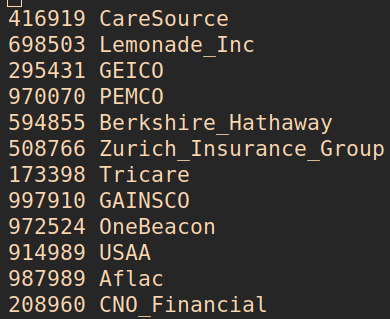
\includegraphics[width=0.6\textwidth]{pictures/gen_file.png}
  \caption{Пример сгенерированного файла (первые строки)}
  \label{fig:search_data}
\end{figure}
\subsection{Тестирование программы}
Для того чтобы убедиться, что генератор записей работает верно произведем
тестирование функций (табл. \ref{tab:task1_test}).
\begin{table}[htpb]
  \centering
  \caption{Тестирование задачи 1}
  \label{tab:task1_test}
  \begin{tabular}{|c|c|c|c|}
    \hline
    \parbox[c]{15mm}{\centering Номер \\ теста} & Входные данные &
    \parbox[m]{3cm}{\centering Ожидаемый \\ результат} &
    \parbox[m]{6cm}{\centering Результат \\ выполнения программы \\(размер файла)}
    \\ \hline
    1 & \parbox[c]{5cm}{\centering 10}
      & \parbox[m]{3cm}{\centering $\approx$190 байт} & \raisebox{-.5\height}
      {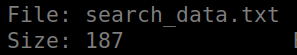
\includegraphics[width=65mm, height=12mm]{pictures/task1_test1.png}} \\ \hline
    2 & \parbox[c]{5cm}{\centering 100}
      & \parbox[m]{3cm}{\centering $\approx$1900 байт} & \raisebox{-.5\height}
      {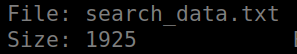
\includegraphics[width=65mm, height=12mm]{pictures/task1_test2.png}} \\ \hline
    3 & \parbox[c]{5cm}{\centering 1000}
      & \parbox[m]{3cm}{\centering $\approx$19000 байт } & \raisebox{-.5\height}
      {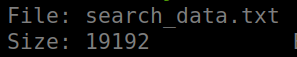
\includegraphics[width=65mm, height=12mm]{pictures/task1_test3.png}} \\ \hline
  \end{tabular}
\end{table}
\newpage
\section{Задание 2}
\subsection{Постановка задачи}
Разработать программу поиска записи по ключу в текстовом файле с
применением алгоритма линейного поиска.
\subsection{Алгоритм линейного поиска}
Параметры функции: file\_name - имя файла, в котором будет производиться
поиск; key - ключ, по которому будет производиться поиск.
Остальные переменные описаны в комментариях алгоритма.
\begin{algorithm}
  \floatname{algorithm}{Алгоритм}
  \caption{Алгоритм функции линейного поиска}
  \label{alg:linear_search_algo}
  \begin{algorithmic}
    \Function{linearSearchFile}{file\_name, key}
    \State Let's fin - input file stream \Comment Поток чтения из файла
    \State fin.open(file\_name)
    \State Let's line - string \Comment Текущая прочитанная запись
    \While{std::getline(fin, line)}
    \If{key in the line equals key in the parameter}
    \State \Return line
    \EndIf
    \EndWhile
    \State \Return "no\_line" \Comment Запись не найдена
    \EndFunction
  \end{algorithmic}
\end{algorithm}
\subsection{Код функции поиска}
linearSearchFile:
\begin{itemize}
  \item Предусловие - файл с указанным именем существует и запись с указанным
    ключом существует (по условию задачи)
  \item Постусловие - возвращена запись с указанным ключом 
\end{itemize}
\lstinputlisting[lastline=27]{code/search_algos.cpp}
\subsection{Код программы}
Код файла main\_first.cpp:
\lstinputlisting{code/main_first.cpp}
\subsection{Тестирование программы}
Для того чтобы убедиться, что функция линейного поиска работает верно
произведем тестирование функции (таблица \ref{tab:task2_test}).
\begin{table}[htpb]
  \centering
  \caption{Тестирование задачи 2}
  \label{tab:task2_test}
  \begin{tabular}{|c|c|c|c|}
    \hline
    \parbox[c]{15mm}{\centering Номер \\ теста} & Входные данные &
    \parbox[m]{3cm}{\centering Ожидаемый \\ результат} &
    \parbox[m]{6cm}{\centering Результат \\ выполнения программы}
    \\ \hline
    1 & \parbox[c]{5cm}{\centering 673124}
      & \parbox[m]{3cm}{\centering 673124 Primerica} & \raisebox{-.5\height}
      {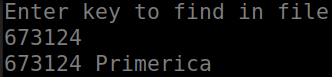
\includegraphics[width=65mm, height=15mm]{pictures/task2_test1.png}} \\ \hline
    2 & \parbox[c]{5cm}{\centering 451098}
      & \parbox[m]{3cm}{\centering 451098 Erie\_\\Insurance\_\\Group} & \raisebox{-.5\height}
      {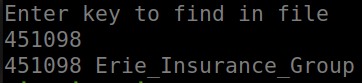
\includegraphics[width=65mm, height=15mm]{pictures/task2_test2.png}} \\ \hline
    3 & \parbox[c]{5cm}{\centering 912836}
      & \parbox[m]{3cm}{\centering 912836 Liberty\_Mutual} & \raisebox{-.5\height}
      {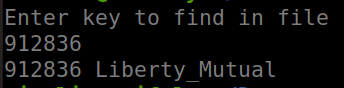
\includegraphics[width=65mm, height=15mm]{pictures/task2_test3.png}} \\ \hline
  \end{tabular}
\end{table}

\subsection{Замера времени работы функции}
Чтобы оценить скорость работы функции линейного поиска произведем
тестирование функции с замером времени. Тестирование будет производится на
файлах из 100 и 1000 записей. В функцию будут передаваться последовательно
ключи 3-х записей – записи, расположенной в начале, в середине и в конце файла.
Результаты тестирования приведены в таблице \ref{tab:task2_speed}.
\begin{table}[htpb]
  \centering
  \caption{Тестирования скорости алгоритма задачи 2}
  \label{tab:task2_speed}
  \begin{tabular}{|p{3cm}|p{6cm}|p{6cm}|}
    \hline
    Расположение записи & Время поиска в файле из 100 записей
                        & Время поиска в файле из 1000 записей
    \\ \hline
    Начало & \raisebox{-.5\height}{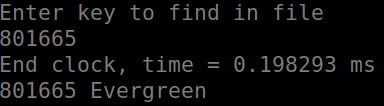
\includegraphics[width=60mm, height=20mm]{pictures/task2_speed1_1.png}}
           & \raisebox{-.5\height}{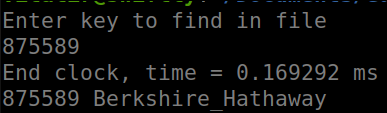
\includegraphics[width=60mm, height=20mm]{pictures/task2_speed2_1.png}}
    \\ \hline
    Середина & \raisebox{-.5\height}{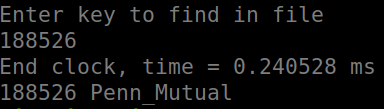
\includegraphics[width=60mm, height=20mm]{pictures/task2_speed1_2.png}}
           & \raisebox{-.5\height}{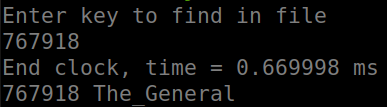
\includegraphics[width=60mm, height=20mm]{pictures/task2_speed2_2.png}}
    \\ \hline
    Конец  & \raisebox{-.5\height}{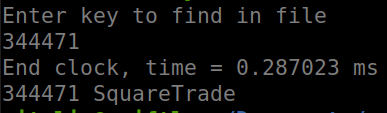
\includegraphics[width=60mm, height=20mm]{pictures/task2_speed1_3.png}}
           & \raisebox{-.5\height}{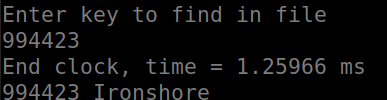
\includegraphics[width=60mm, height=20mm]{pictures/task2_speed2_3.png}}
    \\ \hline
  \end{tabular}
\end{table}
\newpage
\section{Задание 3}
\subsection{Постановка задачи}
Разработать функцию интерполяционного поиска записи в файле.
\subsection{Описание алгоритма доступа к записи в файле посредством таблицы}
Таблица будет представлять собой массив строк в порядке аналогичном
записям в файле. Ссылкой на запись будет являться индекс элемента, по которому
будет выводится соответствующая запись файла.
\subsection{Алгоритм интерполяционного поиска}
Параметры функции: rows - вектор из прочитанных записей, в котором будет производиться
поиск; key - ключ, по которому будет производиться поиск.
Остальные переменные описаны в комментариях алгоритма.
\newpage
\begin{algorithm}
  \floatname{algorithm}{Алгоритм}
  \caption{Алгоритм функции интерполяционного поиска}
  \label{alg:interpolation_search_algo}
  \begin{algorithmic}
    \Function{interpolationSearch}{rows, key}
    \State low $\gets$ 0 \Comment Нижняя граница поиска
    \State high  $\gets$ the size of the rows - 1 \Comment Верхняя граница поиска
    \State mid  $\gets$ 0 \Comment Центр поиска
    \While{rows[high] != rows[low] and key $\geq $ key of the rows[low]
    and key $\leq $ key of the rows[high]}
    \State mid $\gets$ low + (key - key of the rows[low]) * (high - low)
    / (key of the rows[high] - key of the rows[low]))
    \If{key of the rows[mid] < key}
    \State low $\gets$ mid + 1
    \ElsIf{key of the rows[mid] > key}
    \State high  $\gets$ mid - 1
    \Else
    \State \Return rows[mid] 
    \EndIf
    \EndWhile
    \If{key == key of the rows[low]}
    \State \Return rows[low]
    \Else
    \State \Return "no\_key"
    \EndIf
    \EndFunction
  \end{algorithmic}
\end{algorithm}
\subsection{Код функции поиска}
interpolationSearch:
\begin{itemize}
  \item Предусловие - файл с указанным именем существует и запись с указанным
    ключом существует (по условию задачи)
  \item Постусловие - возвращена запись с указанным ключом 
\end{itemize}
\lstinputlisting[firstline=28]{code/search_algos.cpp}
\subsection{Код программы}
Код файла main\_second.cpp:
\lstinputlisting{code/main_second.cpp}
\subsection{Тестирование программы}
Для того чтобы убедиться, что функция интерполяционного поиска работает верно
произведем тестирование функции (таблица \ref{tab:task3_test}).
\begin{table}[htpb]
  \centering
  \caption{Тестирование задачи 3}
  \label{tab:task3_test}
  \begin{tabular}{|c|c|c|c|}
    \hline
    \parbox[c]{15mm}{\centering Номер \\ теста} & Входные данные &
    \parbox[m]{3cm}{\centering Ожидаемый \\ результат} &
    \parbox[m]{6cm}{\centering Результат \\ выполнения программы}
    \\ \hline
    1 & \parbox[c]{5cm}{\centering 132343}
      & \parbox[m]{3cm}{\centering 132343 FM\_Global} & \raisebox{-.5\height}
      {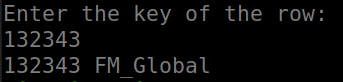
\includegraphics[width=65mm, height=15mm]{pictures/task3_test1.png}} \\ \hline
    2 & \parbox[c]{5cm}{\centering 574851}
      & \parbox[m]{3cm}{\centering 574851 Primerica} & \raisebox{-.5\height}
      {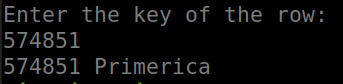
\includegraphics[width=65mm, height=15mm]{pictures/task3_test2.png}} \\ \hline
    3 & \parbox[c]{5cm}{\centering 988153}
      & \parbox[m]{3cm}{\centering 988153 Allstate} & \raisebox{-.5\height}
      {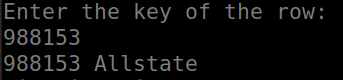
\includegraphics[width=65mm, height=15mm]{pictures/task3_test3.png}} \\ \hline
  \end{tabular}
\end{table}
\subsection{Замера времени работы функции}
Чтобы оценить скорость работы функции интерполяционного поиска произведем
тестирование функции с замером времени. Тестирование будет производится на
файлах из 100 и 1000 записей. В функцию будут передаваться последовательно
ключи 3-х записей – записи, расположенной в начале, в середине и в конце файла.
Результаты тестирования приведены в таблице \ref{tab:task3_speed}.
% I compile these programs (in my report) without optimization
\begin{table}[htpb]
  \centering
  \caption{Тестирования скорости алгоритма задачи 3}
  \label{tab:task3_speed}
  \begin{tabular}{|p{3cm}|p{6cm}|p{6cm}|}
    \hline
    Расположение записи & Время поиска в файле из 100 записей
                        & Время поиска в файле из 1000 записей
    \\ \hline
    Начало & \raisebox{-.5\height}{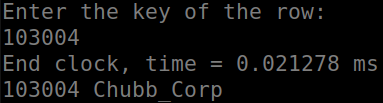
\includegraphics[width=60mm, height=20mm]{pictures/task3_speed1_1.png}}
           & \raisebox{-.5\height}{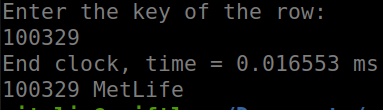
\includegraphics[width=60mm, height=20mm]{pictures/task3_speed2_1.png}}
    \\ \hline
    Середина & \raisebox{-.5\height}{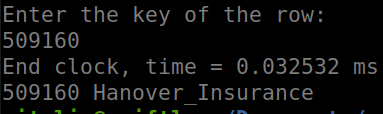
\includegraphics[width=60mm, height=20mm]{pictures/task3_speed1_2.png}}
           & \raisebox{-.5\height}{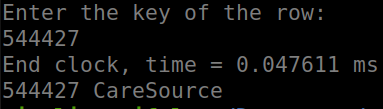
\includegraphics[width=60mm, height=20mm]{pictures/task3_speed2_2.png}}
    \\ \hline
    Конец  & \raisebox{-.5\height}{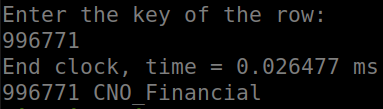
\includegraphics[width=60mm, height=20mm]{pictures/task3_speed1_3.png}}
           & \raisebox{-.5\height}{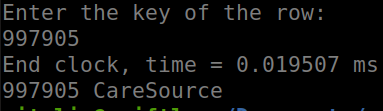
\includegraphics[width=60mm, height=20mm]{pictures/task3_speed2_3.png}}
    \\ \hline
  \end{tabular}
\end{table}

\section{Анализ эффективности алгоритмов поиска}
Произведем анализ эффективности рассмотренных алгоритмов поиска в
файле. Как видно из результатов замера времени для каждого алгоритма
(см. таблицу \ref{tab:general_speed} - общая таблица скоростей, составленная
по таблицам \ref{tab:task2_speed} и \ref{tab:task3_speed}),
алгоритм интерполяционног поиска гораздо быстрее, чем алгоритм линейного поиска.
Алгоритм интерполяционного поиска
меньше зависит от длины массива и во многих частных случаях показывает себя
быстрее (если элемент расположен в самой середине списка).
\begin{table}[htpb]
  \centering
  \caption{Таблица сравнения скоростей алгоритмов}
  \label{tab:general_speed}
  \begin{tabular}{|p{30mm}|p{45mm}|p{2cm}|p{2cm}|p{2cm}|}
    \hline
    \multirow{2}*{Кол-во записей}
    & \multirow{2}*{Алгоритм поиска}
    & \multicolumn{3}{|c|}{\centering Расположение}
    \\ \cline{3-5}
    & & Начало & Середина & Конец
    \\\hline
    \multirow{2}*{100} & Линейный & 0.198 ms & 0.241 ms & 0.287 ms
    \\[20pt] \cline{2-5}
                       & Интерполяционный & 0.021 ms & 0.033 ms & 0.026 ms
    \\[20pt] \hline
    \multirow{2}*{1000} & Линейный & 0.169 ms & 0.670 ms & 1.260 ms
    \\[20pt] \cline{2-5}
                       & Интерполяционный & 0.017 ms & 0.048 ms & 0.020 ms
    \\[20pt] \hline
  \end{tabular}
\end{table}
\newpage
\section*{Выводы}
\addcontentsline{toc}{section}{Выводы}
% Some water by the idea of Esaev Semyon
В ходе данной практической работы были получены знания и практические навыки
по разработке и реализации алгоритмов поиска в таблице данных.
Также были опробованы применения алгоритмов поиска к поиску по ключу
записей в файле, а также получен практический опыт по применению
алгоритмов поиска в таблицах данных. В первом
задании был разработан генератор таблицы данных в соответствии с вариантом
индивидуального задания, а также описаны прототипы используемых функций и
протестирован алгоритм. Во втором задании был разработан алгоритм линейного
поиска, описаны функции, протестирован алгоритм и произведён замер времени для
разных случаев поиска. В третьем задании был разработан алгоритм интерполяционного поиска,
протестирован и произведен замер времени для разных случаев. На основе замеров
времени были проанализированы эффективности изученных алгоритмов и получен вывод, %
что алгоритм интерполяционного поиска является более эффективным, чем алгоритм
линейного поиска.
\section*{Список информационных источников}
\addcontentsline{toc}{section}{Список информационных источников}
\begin{enumerate}[leftmargin=*]
  \item Thomas H. Cormen, Clifford Stein и другие: Introduction to Algorithms, 3rd Edition.
    Сентябрь 2009. The MIT Press.
  \item N. Wirth: Algorithms and Data Structures. Август 2004.
    \\ https://people.inf.ethz.ch/wirth/AD.pdf.
  \item Interpolation search ~//~Wikipedia \\~
    [Электронный ресурс]. URL:
    \\ https://en.wikipedia.org/wiki/Interpolation\_search
    (Дата обращения: 08.05.2021)
   \item Курс Algorithms, part 2 // Coursera [Электронный ресурс]. URL:
     \\ https://www.coursera.org/learn/algorithms-part2
     (Дата обращения: 08.05.2021)
\end{enumerate}
\end{document}
